\documentclass[12pt]{article}
\usepackage{multirow}
\usepackage[english]{babel}
\usepackage[utf8x]{inputenc}
\usepackage{amsmath}
\usepackage{graphicx}
\usepackage[a4paper]{geometry}

\begin{document}
\begin{titlepage}

% definition of custom command for horizontal lines
\newcommand{\HRule}{\rule{\linewidth}{0.5mm}}

\center
% HEADING
\textsc{\LARGE University of Dublin,\\Trinity College}\\[1.0cm]

\includegraphics[width=0.2\textwidth]{logo.png}

\HRule \\[0.4cm]
\textsc{\Large ST2004 Optional Assignment}\\[0.25cm]
\textsc{\large Investigation into Probabilistic Processes of Monopoly}\\[0.1cm]
\HRule \\[0.4cm]
 
% AUTHORS
\begin{minipage}{0.5\textwidth}
\begin{flushleft} \large
\emph{Author:}
\\Edmond \textsc{O'Flynn} 12304742
\end{flushleft}
\end{minipage}
~
\begin{minipage}{0.4\textwidth}
\begin{flushleft} 
\large
\emph{Lecturer:} \\
Brett \textsc{Houlding} 
\end{flushleft}
\end{minipage}\\[3cm]

% DATE
{\large \today}\\[2cm] 

% LOGO
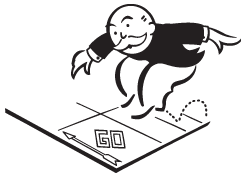
\includegraphics[width=0.4\textwidth]{monopoly_man.png}
\clearpage
\end{titlepage}

\newgeometry{top=1cm,left=1cm,bottom=2cm,right=1cm}
\tableofcontents
\thispagestyle{empty}
\cleardoublepage
\setcounter{page}{1}

\newgeometry{top=2.5cm,left=2.5cm,bottom=2.5cm,right=2.5cm}

\section{Introduction}
\subsection{What is Monopoly?}
Monopoly is a game where players traverse a board across 40 squares consisting of properties, which players may choose to purchase, as well as other spaces that offer chances and opportunities. Whilst the players move around the board with respect to independent dice rolls, the player may choose to buy and improve properties, or to pay rent to other players. The ultimate goal in the game is to cause the other players to become bankrupt, and to be the tycoon of the board. In this investigation, the American board's layout and tiles will be referred to. I will be investigating the probabilistic outcome of landing on given tiles, proving that not all spaces are equally distributed, as well as expansions related to this exploitation.
\begin{figure}[h]
\centering
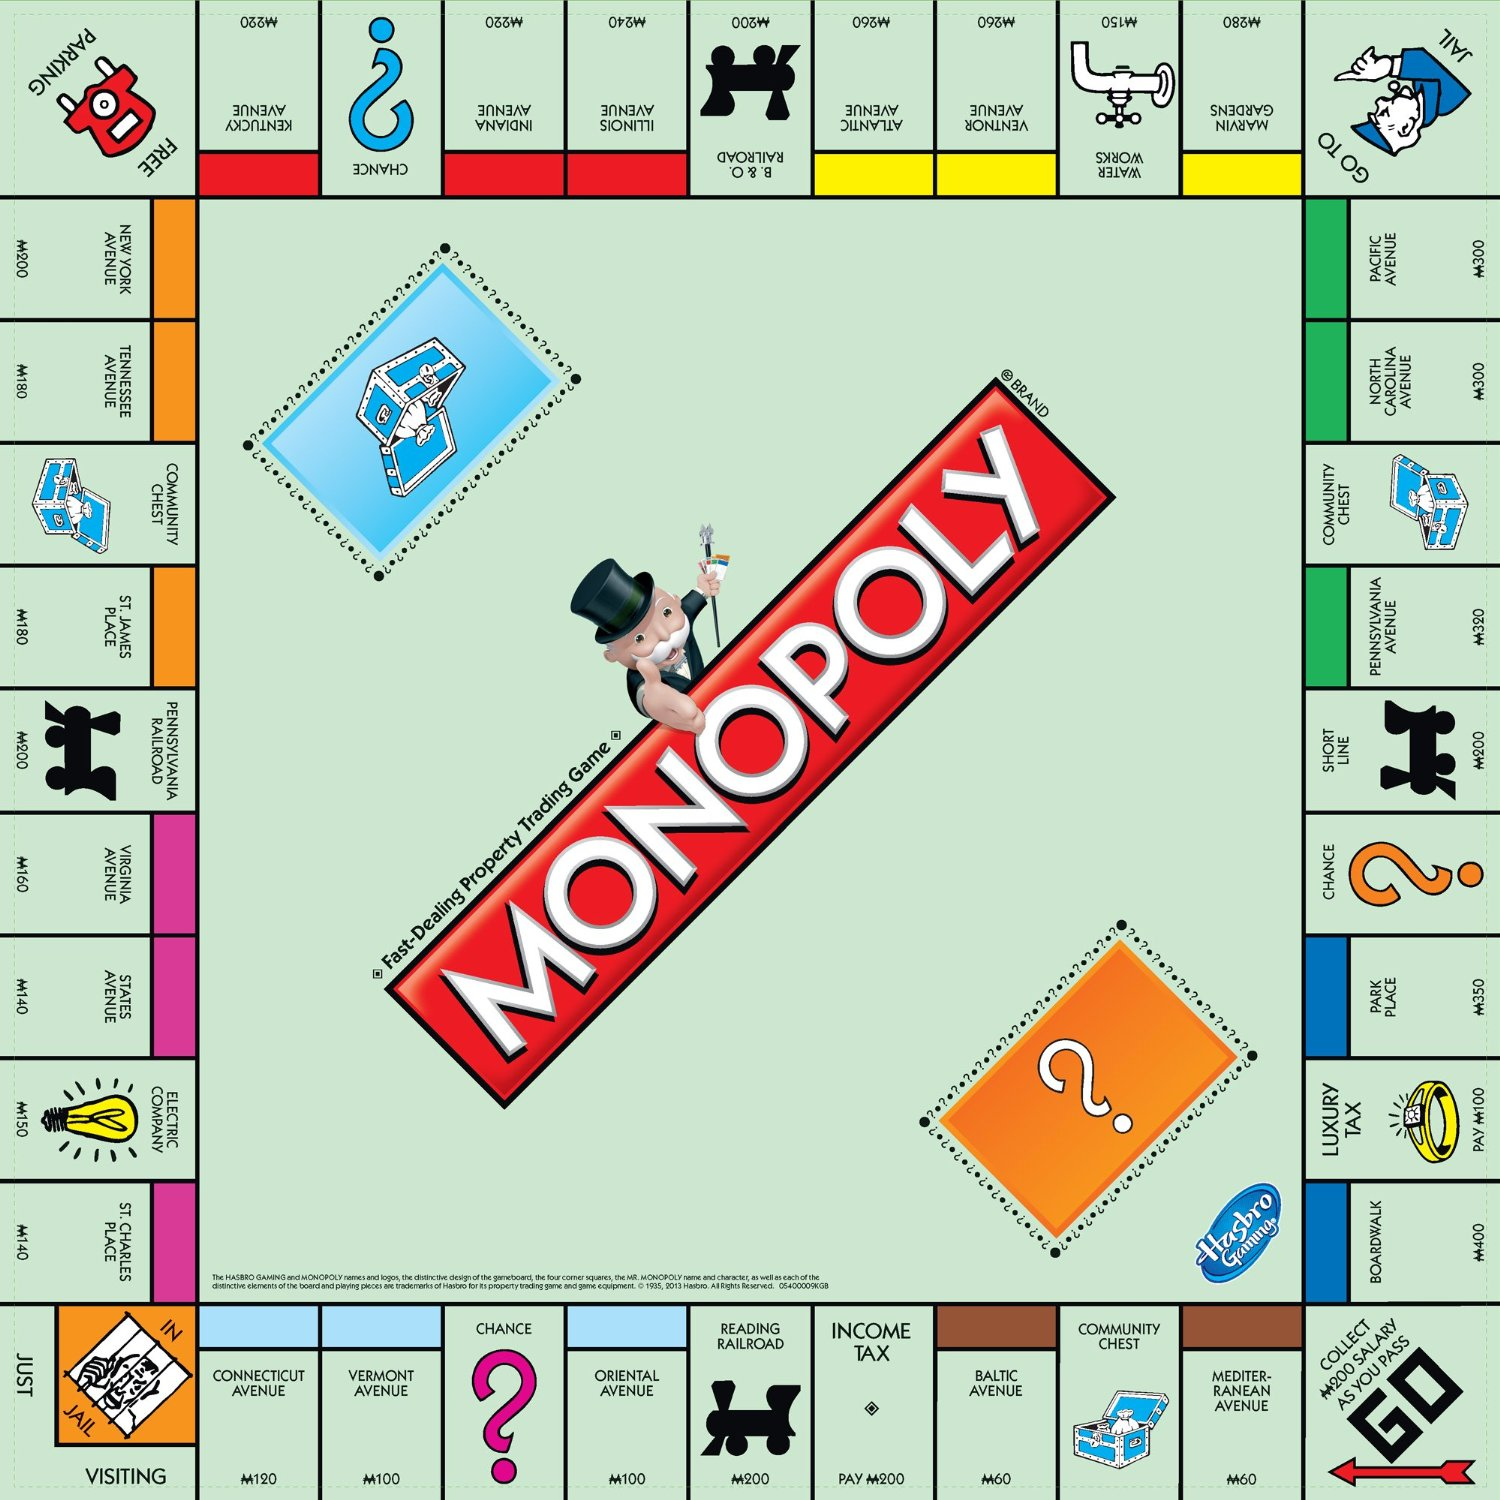
\includegraphics[width=0.6\textwidth]{board.jpg}
\caption{Monopoly board}
\end{figure}
\subsection{Rules}
Monopoly board traversal is the result of fundamentally rolling two independent dice and offsetting by the sum of the dice to the next end square. 
\begin{enumerate}
  \item \textbf{Players start at Go} \hfill \\
  The player moves with respect to the sum of the dice faces clockwise around the board. If a player rolls a double, ie \{1,1\}, \{2,2\} ... \{6,6\}, the player may roll again.
  \item \textbf{Players Can Get Sent to Jail} \hfill \\
  On landing on a space, picking up a specific card, or rolling three doubles in a row, players may get sent to the jail tile.
  \item \textbf{Players May Buy Properties} \hfill \\
  On landing on a non-special tile, a player may choose to buy the land and receive rent if other players land on it. Players may also develop their properties if and only if they possess all colours within that tile group.
  \item \textbf{Winning Conditions} \hfill \\
  A player is deemed the winner if the other players become bankrupt, and only one player is left standing.
\end{enumerate}
\section{Model \& Simulation Background Theory}
\subsection{Dice Rolls}
\begin{table}[h]
\centering
\label{Dice Roll Outcomes}
\begin{tabular}{cccccc}
(1,1) & (1,2) & (1,3) & (1,4) & (1,5) & (1,6) \\
(2,1) & (2,2) & (2,3) & (2,4) & (2,5) & (2,6) \\
(3,1) & (3,2) & (3,3) & (3,4) & (3,5) & (3,6) \\
(4,1) & (4,2) & (4,3) & (4,4) & (4,5) & (4,6) \\
(5,1) & (5,2) & (5,3) & (5,4) & (5,5) & (5,6) \\
(6,1) & (6,2) & (6,3) & (6,4) & (6,5) & (6,6)
\end{tabular}
\caption{Dice Roll Outcomes}
\end{table}
Given that a double has not been rolled on the first turn of the game, the following is the probabilistic outcome of landing on a square from starting position.

\begin{figure}[h]
\centering
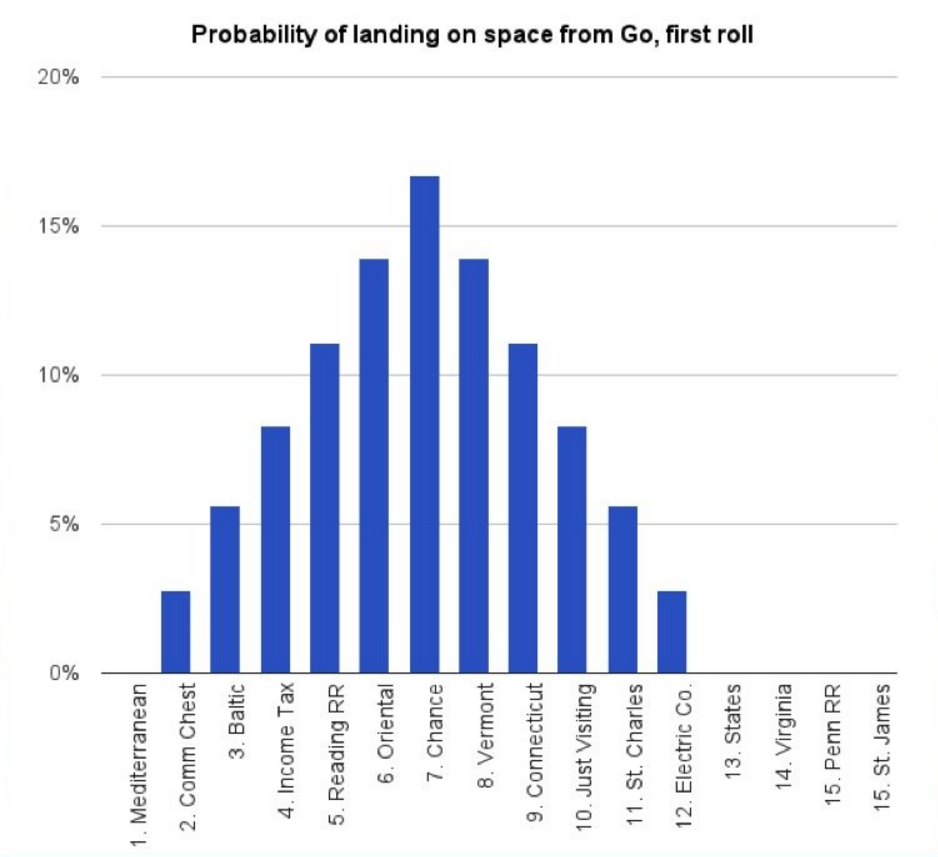
\includegraphics[width=0.5\textwidth]{non_doubles_go.png}
\caption{Distribution of Dice without Doubles Rule from Go}
\end{figure}
\begin{figure}[h]
\centering
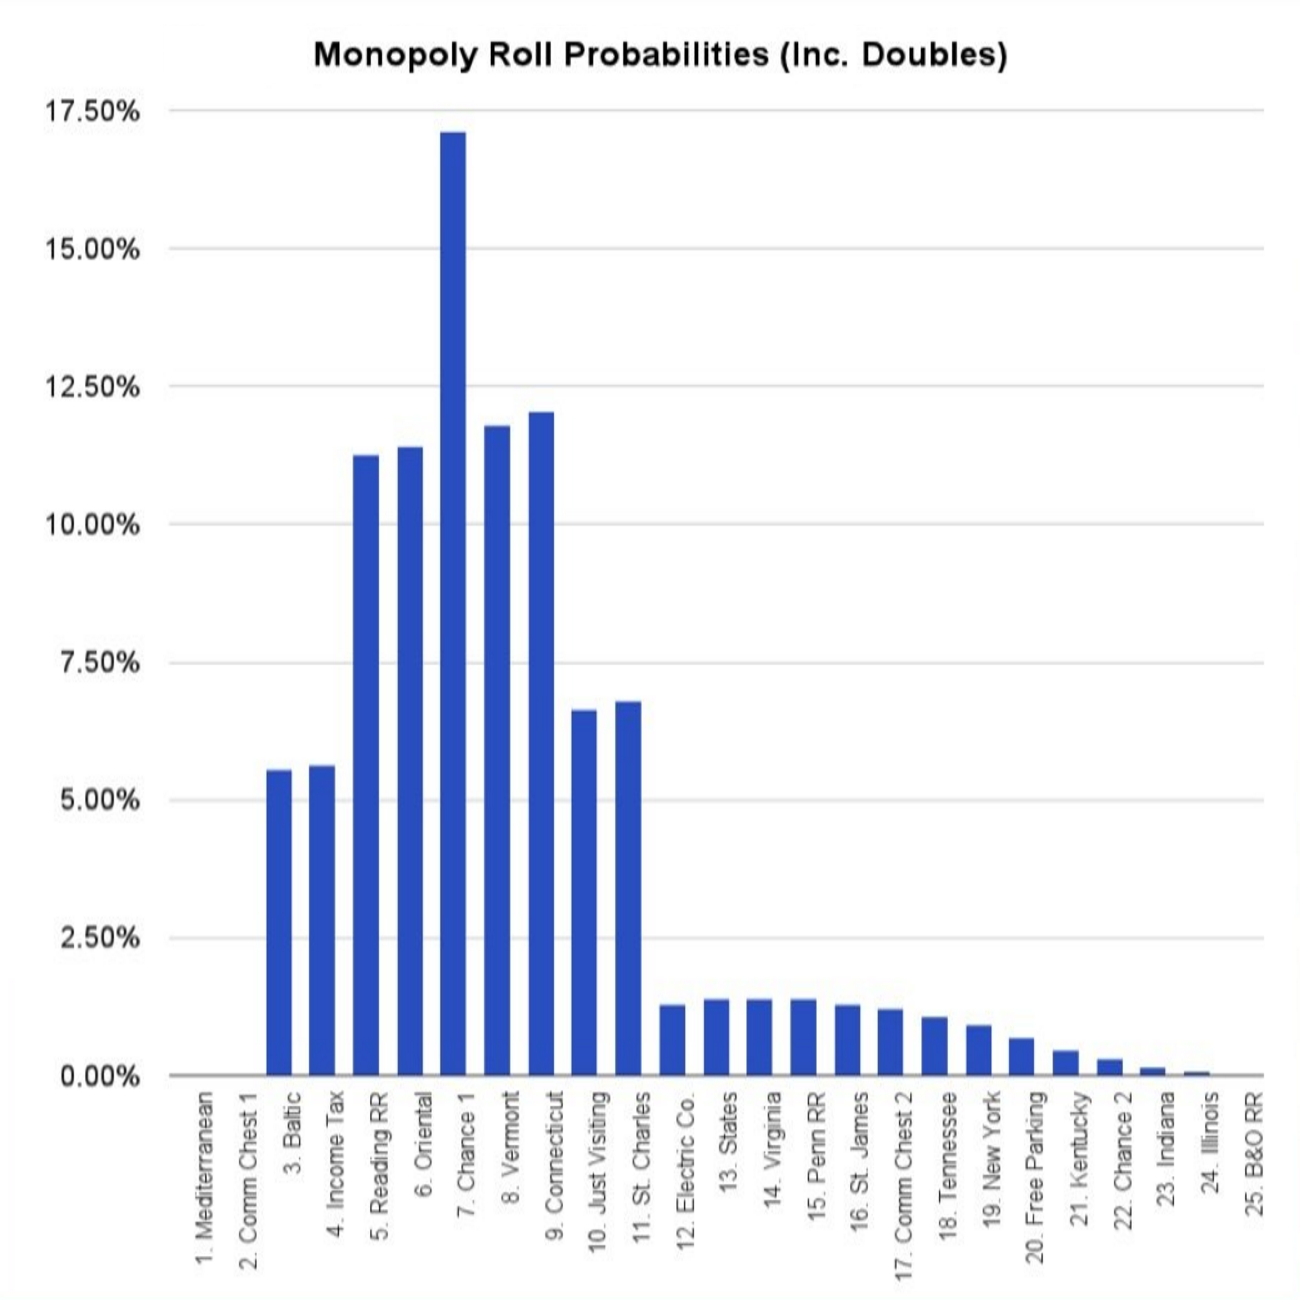
\includegraphics[width=0.5\textwidth]{incl_doubles_go.png}
\caption{Distribution of Dice Including Doubles Rule from Go}
\end{figure}
Given that the outcome was not a double, there is a significantly higher chance of landing on a chance square, which is comparatively higher than landing on squares Oriental Ave or Vermont Ave. Comparatively so, there is still a higher than 10\% chance of landing on squares 5-9.
\begin{figure}[h]
\centering
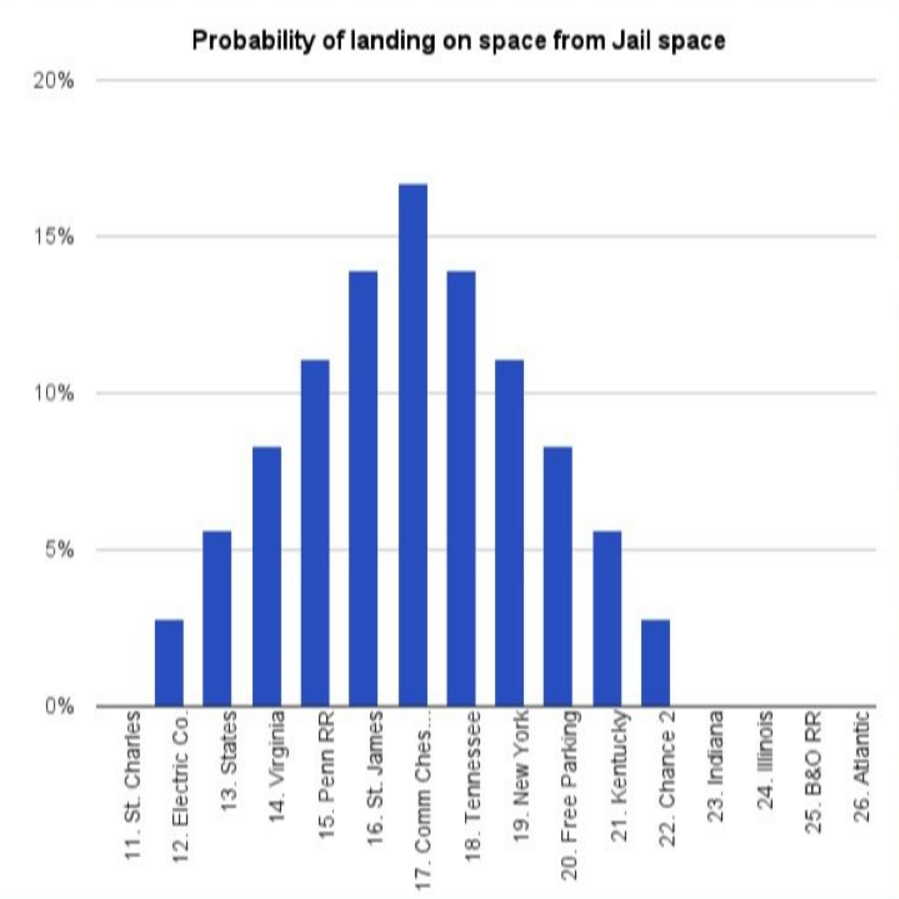
\includegraphics[width=0.5\textwidth]{non_doubles_jail.png}
\caption{Distribution of Dice without Doubles Rule from Jail}
\end{figure}
\begin{figure}[h]
\centering
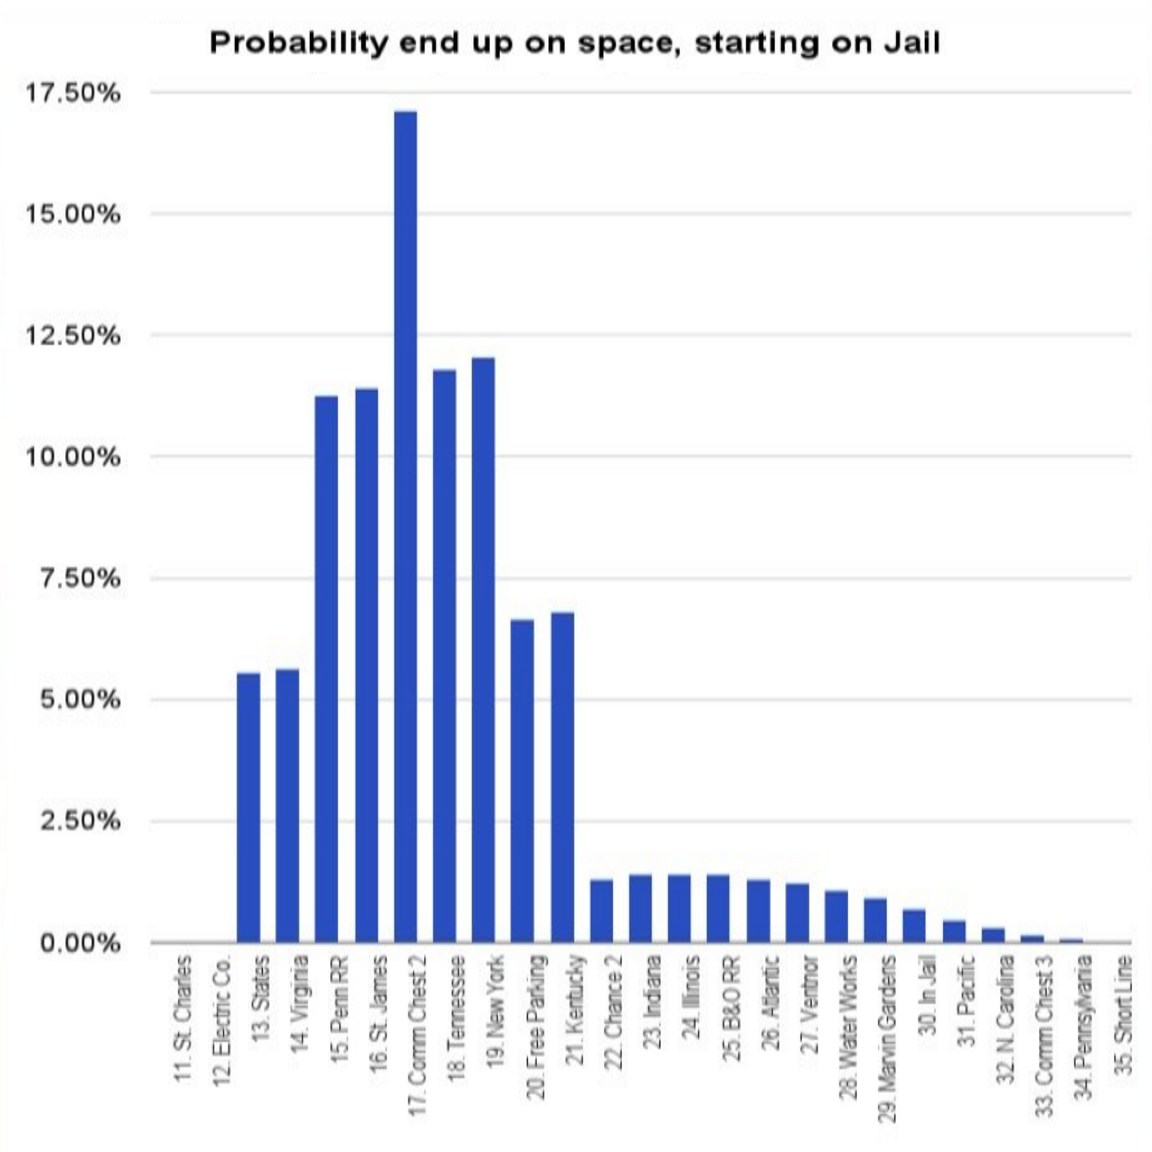
\includegraphics[width=0.5\textwidth]{incl_doubles_jail.png}
\caption{Distribution of Dice without Doubles Rule from Jail}
\end{figure}
Doubles can be extremely powerful, thus changing the probabilistic outcomes of square landing probability, allowing for some tiles to obtain higher and lower frequencies than other tiles over the long run. The Monopoly board itself is a vector of length 40 which recursively loops on itself, containing a mixture of tiles ranging from properties to varying cards that affect the player in different ways, both positively and negatively. 
\begin{figure}[h]
\centering
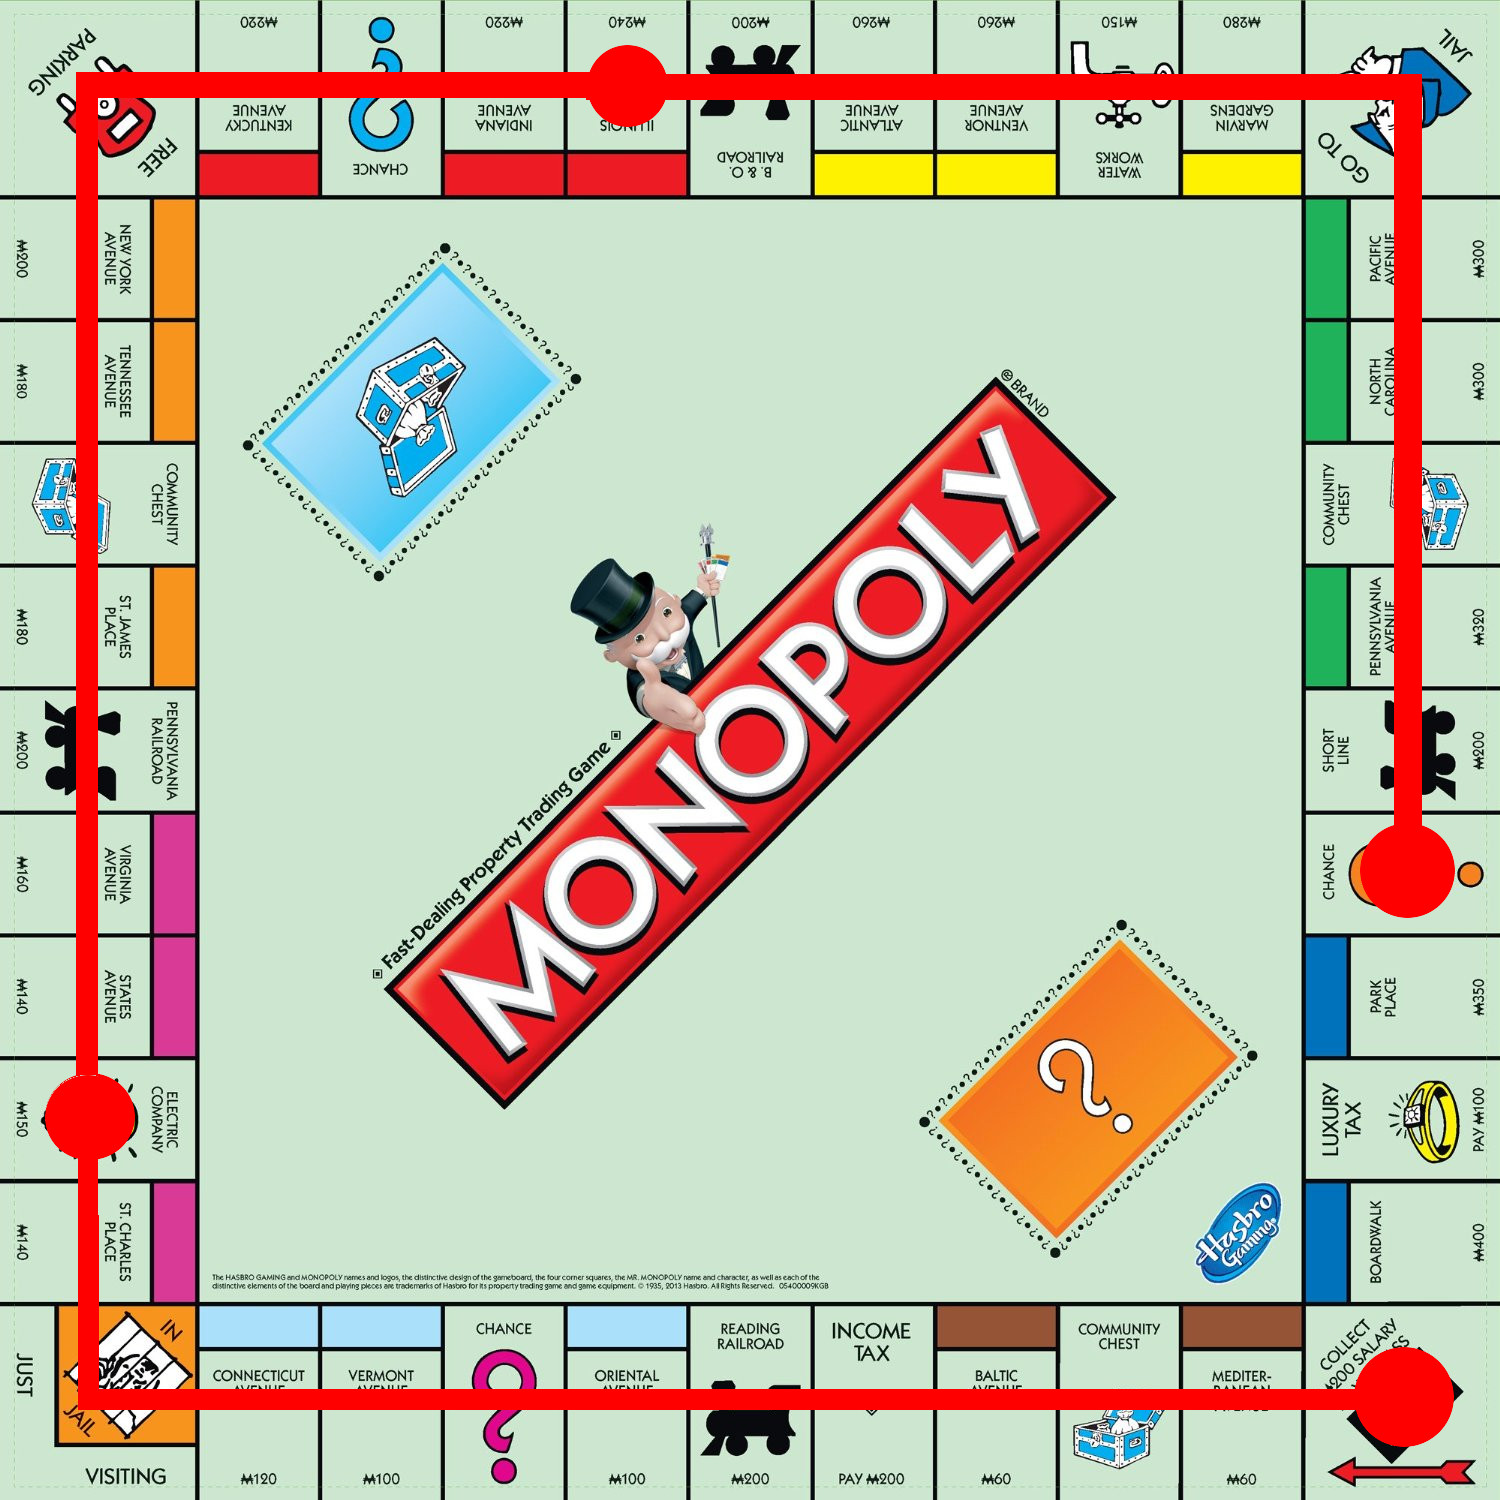
\includegraphics[width=0.5\textwidth]{triple_traverse.jpg}
\caption{Traversing on 3 Double 6s}
\end{figure}
%compare this with the simulation
It is possible to traverse from starting position to the highlighted chance space in one go by rolling 6 6s over 3 turns, its chance of occurrence is exceedingly low, and the player must succumb to the \emph{No Speeding} rule, by which one must go to jail. The chance of rolling three doubles has a $\left(6 \cdot \frac{1}{6} \cdot \frac{1}{6}\right)^3$ , or $0.4\%$, chance of occurrence. Although small, in every 1,000 rolls there will tend to be 4 triple double-rolls thrown and therefore the player gets sent to jail. Rolling 3 double 6s has a chance of $0.0000214\%$ (or $\left(\frac{1}{6}\right)^{6}$) of happening, which is probabilistically extremely unlikely, but still possible with fair dice, where it tends to happen twice in every 100,000 rolls.
\begin{align*}
\frac{1}{6}\approx16.7\% \quad &\textsl{of rolling 1 double}\\
\frac{1}{36}\approx2.8\% \quad &\textsl{of rolling 2 doubles}\\
\frac{1}{216}\approx0.4\% \quad &\textsl{of rolling 3 doubles and ergo get sent to jail} 
\end{align*}
Theoretically it is possible for double-rolls to tend to infinity, albeit exponentially this becomes probabilistically unlikely due to constant decreasing odds as well as the No Speeding rule.
The expected value of rolling 1 die is 3.5, therefore on rolling two dice, it's most likely that the sum of the scores will be 7 as independent events. It's also quite likely that your opponents will roll a 5, 6, 8 or 9 with respect to cumulative probabilities of dice rolling, given the figures above.
\subsection{Chance and Community Chests}
Monopoly contains 16 Community Chest cards, and 16 Chance cards. On landing on a community chest or chance card square, the player must abide by one of the five outcomes of varying probabilities on the cards.

\subsubsection{Chance Cards}
\label{Chance Card Probabilities}
The 32 cards, 16 from Community Chest and 16 from Chance, drastically change the outcome of what happens within a game. By drawing a card from either deck, one of the following five results may happen:
\begin{enumerate}
  \item \textbf{Go to the Stated Tile} \hfill\\
  There is a $\frac{8}{16}$ chance of this.
  \item \textbf{Collect Money} \hfill\\
  There is a $\frac{3}{16}$ chance of this.
  \item \textbf{Pay Money} \hfill\\
  There is a $\frac{3}{16}$ chance of this.
  \item \textbf{Go to Jail} \hfill\\
  There is a $\frac{1}{16}$ chance of this.
  \item \textbf{Get out of Jail} \hfill\\
  There is a $\frac{1}{16}$ chance of this.
\end{enumerate}
Therefore, a probability of $\frac{9}{16}$ cards have the ability to transport the player across the board to another location, thereby altering the odds to being in another place to having a higher probability of landing. There is a total of three possible outcomes of spaces to land on within the weighting effect of certain spaces on the board:

\begin{minipage}{0.5\textwidth}
\begin{flushleft}
\begin{itemize}
  \item {Go to Jail}
  \item {Go Back Three Spaces}
  \item {Advance to Go}
  \item {Advance to Nearest Utility}
\end{itemize}
\end{flushleft}
\end{minipage}
~
\begin{minipage}{0.5\textwidth}
\begin{flushleft} 
\begin{itemize}
  \item {Advance to Nearest Railroad}
  \item {Advance to Boardwalk}
  \item {Advance to Illinois Avenue}
  \item {Advance to Reading Railroad}
  \item {Advance to St. Charles' Place}
\end{itemize}
\end{flushleft}
\end{minipage}
\\
\\
Within the diagram shown, there is a tendency for the game to probabilistically relocate the player more frequently to the first and second rows of the board (due to the selection of cards from Community Chest and Chance), thus creating another weight for frequency on which certain spaces land from card chances alone.

\subsubsection{Community Chest Cards}
\label{Community Chest Probabilities}
The 16 Community Chest cards have similar adverse effect as Chance cards, with the difference that the 5 outcomes have different weightings:
\begin{enumerate}
  \item \textbf{Collect Money} \hfill\\
  There is a $\frac{9}{16}$ chance of this.
  \item \textbf{Pay Money} \hfill\\
  There is a $\frac{4}{16}$ chance of this.
  \item \textbf{Advance to Stated Tile} \hfill\\
  There is a $\frac{1}{16}$ chance of this.
  \item \textbf{Go to Jail} \hfill\\
  There is a $\frac{1}{16}$ chance of this.
  \item \textbf{Get out of Jail} \hfill\\
  There is a $\frac{1}{16}$ chance of this.
\end{enumerate}
Therefore, mathematically it is possible to anticipate the outcomes of certain cards under the weighting of the \emph{Long Run Average}, where the favourability is an abstraction determined on a scale from -2 to +2:

\begin{center}
\label{Card Favourabilities}
\begin{table}[h]
\centering
\begin{tabular}{llllllllllllllll}
\multicolumn{1}{c}{Action} & \multicolumn{1}{c}{Favourability} & \multicolumn{1}{c}{\begin{tabular}[c]{@{}c@{}}Chance Card\end{tabular}} & \multicolumn{1}{c}{\begin{tabular}[c]{@{}c@{}}Community Chest\end{tabular}} &  &  &  &  &  &  &  &  &  &  &  &  \\
\multicolumn{1}{c}{\begin{tabular}[c]{@{}c@{}}Get out of Jail Free\end{tabular}}    & \multicolumn{1}{c}{+2}            & \multicolumn{1}{c}{$\frac{1}{16}$}                                                  & \multicolumn{1}{c}{$\frac{1}{16}$}                                                      &  &  &  &  &  &  &  &  &  &  &  &  \\
\multicolumn{1}{c}{\begin{tabular}[c]{@{}c@{}}Collect  Money\end{tabular}}          & \multicolumn{1}{c}{+1}            & \multicolumn{1}{c}{$\frac{3}{16}$}                                                  & \multicolumn{1}{c}{$\frac{9}{16}$}                                                      &  &  &  &  &  &  &  &  &  &  &  &  \\
\multicolumn{1}{c}{\begin{tabular}[c]{@{}c@{}}Advance to Stated Space\end{tabular}} & \multicolumn{1}{c}{0}             & \multicolumn{1}{c}{$\frac{8}{16}$}                                                  & \multicolumn{1}{c}{$\frac{1}{16}$}                                                      &  &  &  &  &  &  &  &  &  &  &  &  \\
\multicolumn{1}{c}{Pay Money}                                                         & \multicolumn{1}{c}{-1}            & \multicolumn{1}{c}{$\frac{3}{16}$}                                                  & \multicolumn{1}{c}{$\frac{4}{16}$}                                                      &  &  &  &  &  &  &  &  &  &  &  &  \\
\multicolumn{1}{c}{Go to Jail}                                                        & \multicolumn{1}{c}{-2}            & \multicolumn{1}{c}{$\frac{1}{16}$}                                                  & \multicolumn{1}{c}{$\frac{1}{16}$}                                                      \end{tabular}
\caption{Favourability Odds of Cards}
\end{table}
\end{center}
\subsubsection{Exploitation}
Therefore within the confines of Monopoly, it is possible to exploit these weightings in order to buy properties in these areas of higher weightings as well as their neighbouring tiles such that the probabilistic outcome of landing on a space within the vicinity is higher. As previously discussed and shown, the expected value combined with the positioning of Jail and Go allow for properties residing within these areas to have a higher chance of being landed on in comparison to other tiles on the board. Given the expected value of 3.5 per dice where 2 dice are rolled on any given turn, the expected value of the sum of two dice is given to be 7 over the long run.
\subsection{Jail}
\subsubsection{Increasing Odds}
\label{Jail Probabilities}
\begin{align*}
\centering
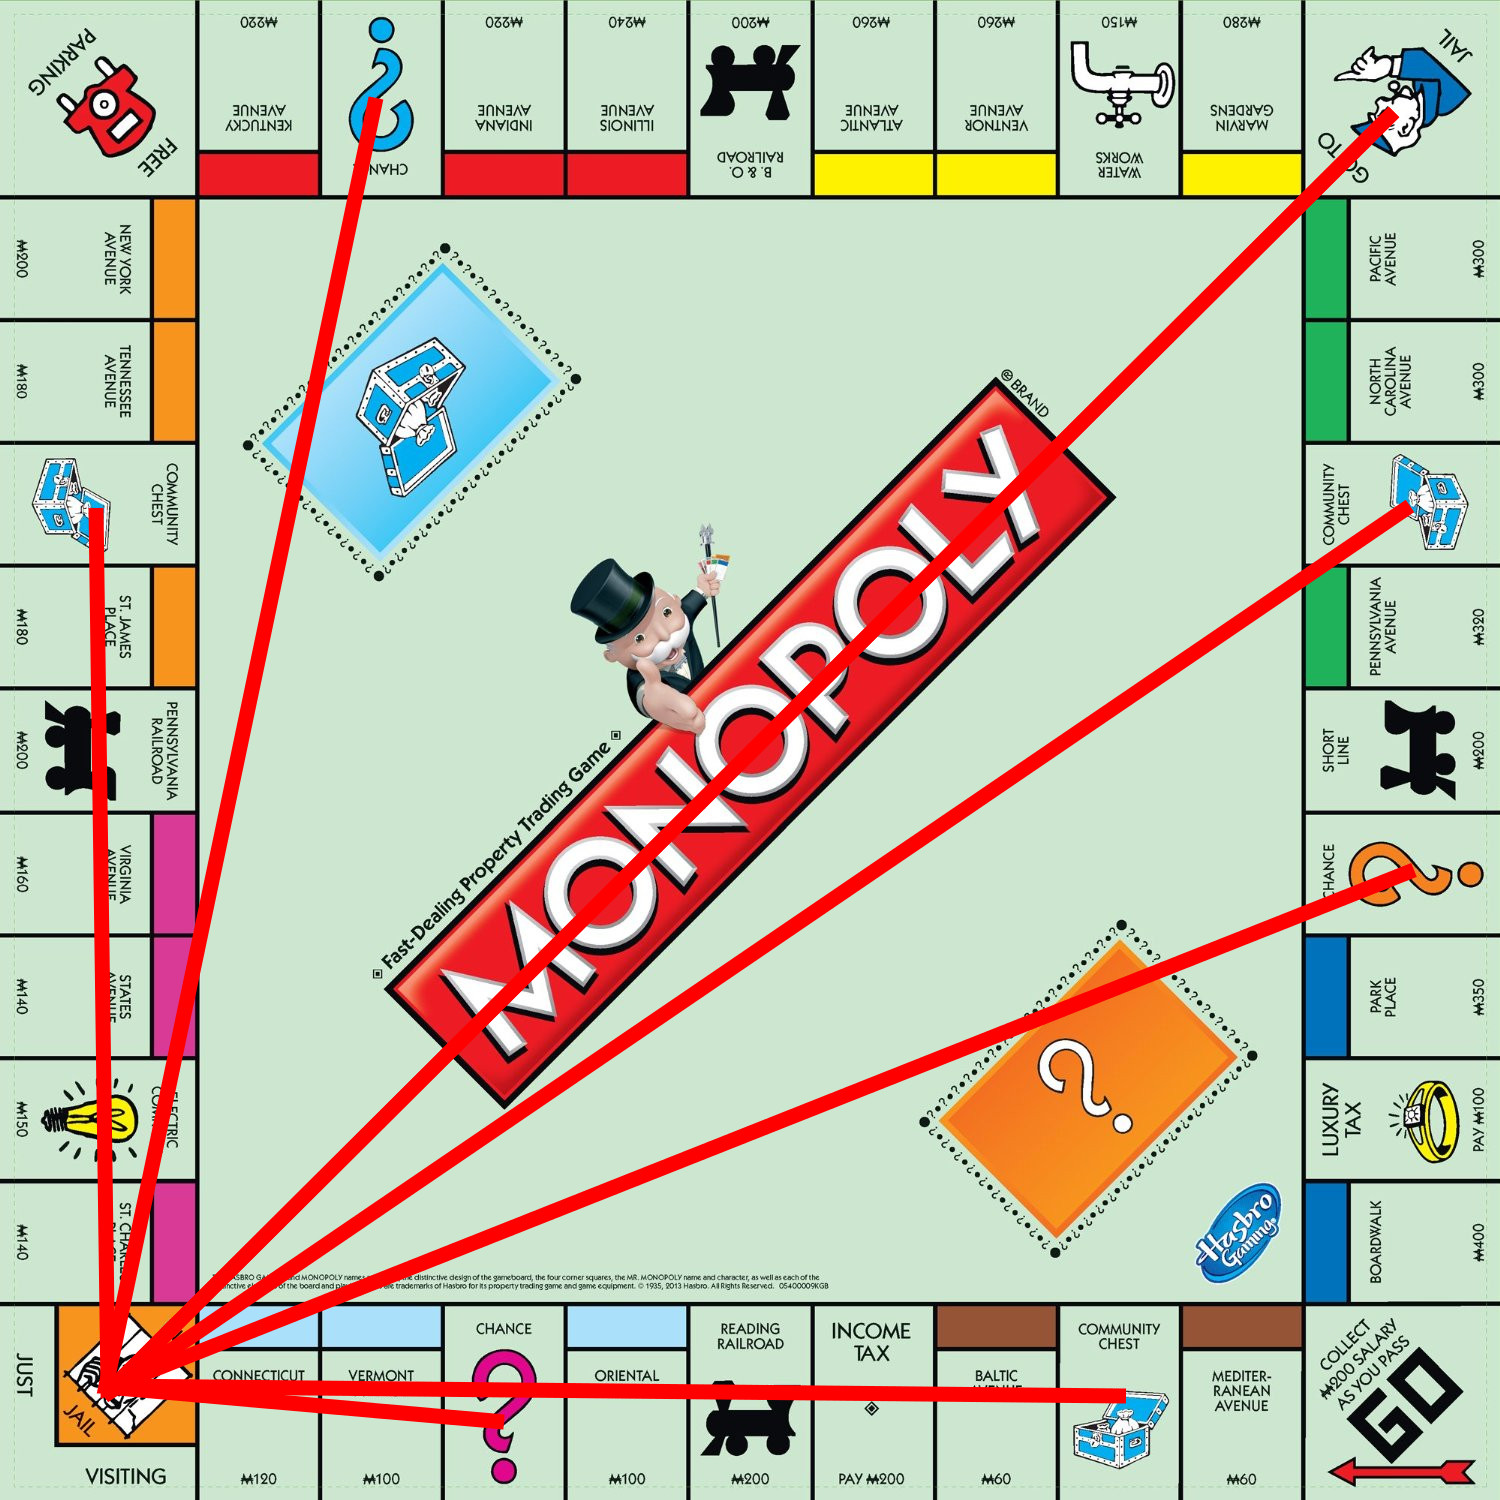
\includegraphics[width=0.6\textwidth]{jail.jpg}
\end{align*}\\
Jail in monopoly acts as a hole on the map into which players are released from at a much higher percentage than any other tile on the map. From here, players emerge, and the expected value of dice causes a shift in dynamics in the field of play. Jail in Monopoly is by far the most probabilistic event within the set of cards of Monopoly's scope. Under regular game conditions, there is a total of 4 reasons for which one may get sent to jail:
\begin{itemize}
  \item {No Speeding Rule on Three Doubles}
  \begin{itemize}
  \item $\frac{1}{216}\approx0.4\%$ chance of occurrence
  \end{itemize}
  \item {Go to Jail Tile}
  \begin{itemize}
  \item $\frac{1}{40}=2.5\%$ chance of occurrence given no tile bias
  \end{itemize}
  \item {Go to Jail Chance Card}
  \begin{itemize}
  \item Chance of occurrence within the deck is $\frac{1}{16}$, or $6.25\%$, and $\frac{1}{16} \cdot \frac{3}{40}$, or $0.47\%$ chance given the amount of Chance cards on the map.
  \end{itemize}
  \item {Go to Jail Community Card}
  \begin{itemize}
  \item Chance of occurrence within the deck is $\frac{1}{16}$, or $6.25\%$, and $\frac{1}{16} \cdot \frac{3}{40}$, or $0.47\%$ chance given the amount of Community Chest cards on the map.
  \end{itemize}
\end{itemize}
\subsubsection{Paradigm}
There is a a set of four different ways to attempt to break custody and escape from jail:
\begin{enumerate}
  \item {Get out of Jail Free Card}\hfill
  \item {Pay \$50 at the Start of a Turn}\hfill
  \item {Roll the Dice and Attempt to Roll a Double} \hfill
  \item {Pay \$50 on Failure to Roll Doubles for the Third Time} \hfill
\end{enumerate}
On success of rolling a double out of jail, the player advances that amount of tiles displayed on the dice from the jail tile. Else on failure to roll a double three times, the player must pay \$50 and again move the total of spaces displayed on the dice from the previous roll. 
The cumulative effect of rolling dice means that over the course of three rolls.
The important probabilistic factor to note is that getting sent to jail is quite a high factor in the scheme of the game, therefore the game has an explicitly hidden factor of game design to route players through the jail tile as both a starting point and a sink.
The probability of rolling out of jail within 3 turns is approximately 42\%, given two independent and fair dice as such:

\begin{table}[h]
\centering
\label{Jail Cumulative Probability}
\begin{tabular}{cccc}
Roll & Process              & Probability & Cumulative Probability \\
1    & $\frac{1}{6}$                  & 16.7\%        & 16.7\%                   \\
2    & $\frac{5}{6}\cdot\frac{1}{6}$         & 13.8\%        & 30.5\%                   \\
3    & $\frac{5}{6}\cdot\frac{5}{6}\cdot\frac{1}{6}$ & 11.8\%        & 42.3\%                  
\end{tabular}
\caption{Cumulative Double Frequency}
\end{table}

This distribution gives rise to what is known as a \emph{Probability Distribution Function}, in which the repeated roll in search of doubles will eventually happen given a long enough series of rolls. The probability of the function tends to 1.
%image here
\section{Markov Chains}
\subsection{What is a Markov Chain?}
Monopoly is based on a 40x40 dimension probability matrix of tiles where each row and column pair represents a space on the board which is subject to a process called a \emph{Markov Chain}. A Markov chain is a probabilistic process in which a steady state probability matrix which is seeded from long term rolls and forecasts. It involves a finite number of states within a finite encapsulation, in this case, the 40 tiles. Markov chains are memoryless, which means that the process in which the player may move freely from tile to tile is independent of the previous tile via dice rolls. Markovian processes are random process whose future probabilities are based only on the current state, and not on the sequence of events preceding the element.

\subsection{Parametrisation}
In order to calculate the probabilities per tile, Monopoly must have a set of Markovian properties calculable by some general factors:
\begin{itemize}
\item Probability vectors
\begin{itemize}
\item A vector with non-negative entries populated to sum to 1.
\end{itemize}
\item Stochastic matrices
\begin{itemize}
\item A square matrix whose columns are populated by probability vectors.
\end{itemize}
\item Steady state vector
\begin{itemize}
\item Adheres to where the sequence $x_0,x_1,...x_n$ is a set of probability vectors whereby the stochastic matrix A is such that $x_{n+1}=Ax_{n}$.
\item Approximates the long term process of the behaviour whereby over subsequent iterations, the Markov Chain tends to $(Ax_{n+1})A=A^2x_{n+1},A^3x_{n+1},...,A^nx_{n+1}$ where $n$ is the period later from the initial time $t$ where in this case, $n=40$ given the transition matrix below.
\end{itemize}
\end{itemize}

\subsubsection{Transition Matrices}
Transition matrices are a stochastic process within Markovian theory where a square matrix is populated by non-negative real numbers whereby each row sums to 1. Given the element in the $i^{th}$ row and $j^{th}$ column, the probability of moving from state \emph{i} to state \emph{j} may be calculated over its long run average within one time step.
\begin{table}[h]
\centering
\label{Transition Matrix}
\begin{tabular}{ccccccc}
                                           &                        & \multicolumn{5}{c}{To}                                                                                                     \\ \cline{3-7} 
                                           & \multicolumn{1}{c|}{}  & \multicolumn{1}{c|}{$1$} & \multicolumn{1}{c|}{$2$} & \multicolumn{1}{c|}{$3$} & \multicolumn{1}{c|}{...} & \multicolumn{1}{c|}{$n$} \\ \cline{2-7} 
\multicolumn{1}{c|}{\multirow{5}{*}{From}} & \multicolumn{1}{c|}{$1$} & \multicolumn{1}{c|}{$a_{1,1}$}  & \multicolumn{1}{c|}{$a_{1,2}$}  & \multicolumn{1}{c|}{$a_{1,3}$}  & \multicolumn{1}{c|}{...}  & \multicolumn{1}{c|}{$a_{1,n}$}  \\ \cline{2-7} 
\multicolumn{1}{c|}{}                      & \multicolumn{1}{c|}{$2$} & \multicolumn{1}{c|}{$a_{2,1}$}  & \multicolumn{1}{c|}{$a_{2,2}$}  & \multicolumn{1}{c|}{$a_{2,3}$}  & \multicolumn{1}{c|}{...}  & \multicolumn{1}{c|}{$a_{2,n}$}  \\ \cline{2-7} 
\multicolumn{1}{c|}{}                      & \multicolumn{1}{c|}{$3$} & \multicolumn{1}{c|}{$a_{3,1}$}  & \multicolumn{1}{c|}{$a_{3,2}$}  & \multicolumn{1}{c|}{$a_{3,3}$}  & \multicolumn{1}{c|}{...}  & \multicolumn{1}{c|}{$a_{3,n}$}  \\ \cline{2-7} 
\multicolumn{1}{c|}{}                      & \multicolumn{1}{c|}{...} & \multicolumn{1}{c|}{...}  & \multicolumn{1}{c|}{...}  & \multicolumn{1}{c|}{...}  & \multicolumn{1}{c|}{...}  & \multicolumn{1}{c|}{...}  \\ \cline{2-7} 
\multicolumn{1}{c|}{}                      & \multicolumn{1}{c|}{$n$} & \multicolumn{1}{c|}{$a_{n,1}$}  & \multicolumn{1}{c|}{$a_{n,2}$}  & \multicolumn{1}{c|}{$a_{n,3}$}  & \multicolumn{1}{c|}{...}  & \multicolumn{1}{c|}{$a_{n,n}$}  \\ \cline{2-7} 
\end{tabular}
\caption{Transition Matrix}
\end{table}
\\
The 1,600 transitional probabilities for all tiles within the Markov sequence are encoded in a 40x40 matrix of the probabilities of moving from one tile to another. Given the states, the transition matrix can be made more complex by extending to 42x42, given the intention to stay in jail for up to 3 turns inclusive.

\subsubsection{Simplified Chains}
In a steady population where the population remains constant, neglecting population changes by immigration, emigration, deaths and births; it is possible to work out the proportions of the population inhabiting each area A, B, and C in which there is a system of change occurring.

For example, assume areas A, B, and C where the following conditions of the system are true on an annual basis of t:
\begin{itemize}
\item Of the population within A, 97\% will stay in A
\begin{itemize}
\item 1\% will more to B from A
\item 1\% will move to C from A
\end{itemize}
\item Of the population within B, 95\% will stay in B
\begin{itemize}
\item 3\% will more to A from B
\item 2\% will move to C from B
\end{itemize}
\item Of the population within C, 96\% will stay in C
\begin{itemize}
\item 3\% will more to A from C
\item 1\% will move to B from C
\end{itemize}
\end{itemize}

\begin{table}[h]
\centering
\begin{tabular}{ccccc}
                      & \multicolumn{4}{c}{To} \\
\multirow{4}{*}{From} &   & A    & B    & C    \\
                      & A & 0.97 & 0.01 & 0.02 \\
                      & B & 0.03 & 0.95 & 0.02 \\
                      & C & 0.03 & 0.01 & 0.96
\end{tabular}
\caption{Transitional Matrix for A, B, and C}
\end{table}

Assuming a population of 1000 in B, given no restrictions on initial population distributions and 0 inhabitants in A and C, time can elapse and the distributive effect of the population spread should be observed, where n is the $n^{th}$ year at which a steady state system has been achieved.

\begin{table}[h]
\centering
\begin{tabular}{cccc}
Year & A       & B       & C       \\
0    & 0       & 1000    & 0       \\
1    & 30      & 950     & 20      \\
2    & 58.2    & 903     & 38.8    \\
...  & ...     & ...     & ...     \\
100  & 499     & 168.4   & 332.6   \\
200  & 499.998 & 166.667 & 333.32  \\
$t \to n$    & $1000\cdot\frac{1}{2}$     & $1000\cdot\frac{1}{6}$  & $1000\cdot\frac{1}{3}$
\end{tabular}
\caption{Long Run Observation within the system}
\end{table} 

Given the system reaches its steady state conditions, the proportions no longer change, and the value at $t+1$, where $t$ has reached steady state, are equivalent in value, therefore

\begin{itemize}
\item $P_A = 0.5$
\item $P_B = 0.166\dot{6}$
\item $P_C = 0.33\dot{3}$
\end{itemize}

Under conditions, generic equations can be formed for the system, where any two of the three states can be solved via algebraic simultaneous equations forming the steady state proportions.

\begin{itemize}
\item $P_A = 0.97 \cdot P_A + 0.03 \cdot P_B + 0.03 \cdot P_C$
\item $P_B = 0.01 \cdot P_A + 0.95 \cdot P_B + 0.01 \cdot P_C$
\item $P_C = 0.02 \cdot P_A + 0.02 \cdot P_B + 0.96 \cdot P_C$
\item $P_A+P_B+P_C=1.000$
\end{itemize}
This process can be extended to Monopoly, where instead of a 3x3 matrix, there is a 40x40 matrix of tiles that is immutable and governs steady state proportions by long run averages.

\subsection{Seeded Matrices}
\subsubsection{Assumptions}
\begin{itemize}
\item On picking up a chance or community chest card, the deck is entirely shuffled in a randomised order having performed the indicated action.
\item Jail escape is a process of only escape with respect to rolling doubles or the effect of having picked up a Get Out of Jail Free card prior to getting sent to the tile.
\item There are three selective states within Monopoly over 40 tiles:
\begin{itemize}
\item 40 tiles in a regular state
\item Doubles rule with the roll again state
\item Community Chest/Chance cards state
\end{itemize}
\item Therefore there are 120 states in Monopoly in any given turn.
\end{itemize}

\subsection{Simulation}
\subsubsection{Set Up}
In order to quickly simulate a game of Monopoly over an exceedingly large amount of rolls, a simulation of the game was programmed in \emph{Java} with respect to assumptions within the Markovian processes, as well as some generified aspects within the pseudo-random rolling process whereby a pseudo-random number was generated twice per turn using different seed values with respect to the current time in milliseconds on my machine. 

\subsubsection{Aspects}
The Monopoly simulation worked on the bases of simplified aspects where 100,000 turns of play were simulated without the aspect of money or other players involved within the turns, therefore taking only cards, jail and dice values into account as per the effects possible per turn. The following is the list of tiles in order of their probability to be landed on which tends to the long run Markovian averages:
\begin{align*}
\centering
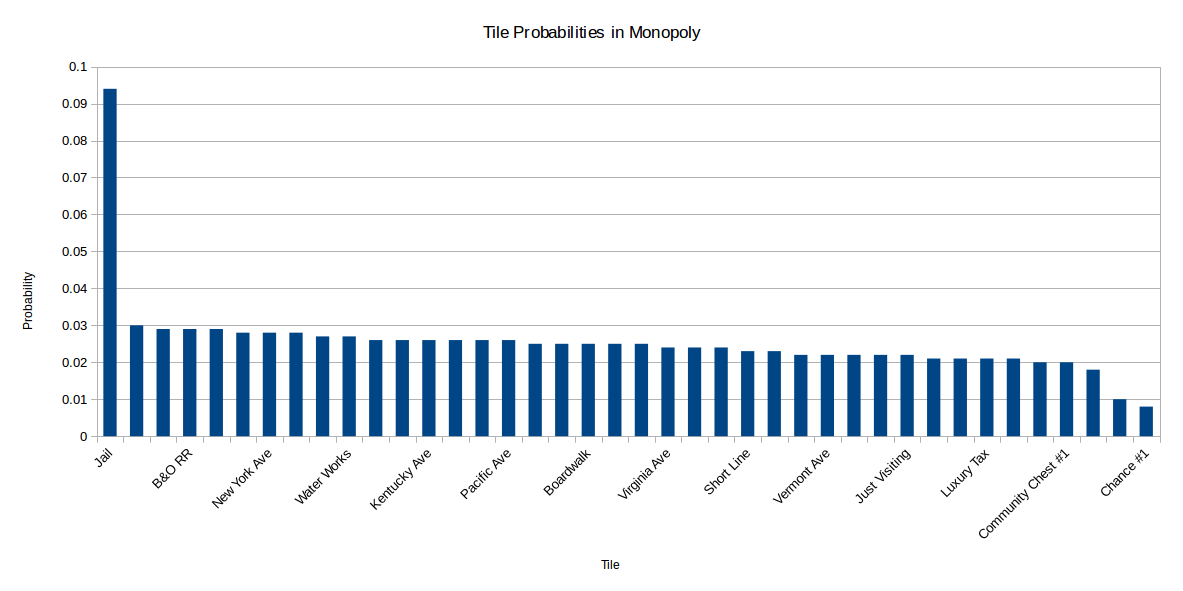
\includegraphics[width=1\textwidth]{tile_prob_graph.png}
\end{align*}
\subsection{Tile Probabilities}
\begin{align*}
\label{Tile Probabilities}
\centering
\begin{minipage}{0.5\textwidth}
\begin{flushleft}
\begin{itemize}
  \item {01. Jail - 0.094}
  \item {02. Illinois Ave - 0.03}
  \item {03. Go - 0.029}
  \item {04. B\&O RR - 0.029}
  \item {05. Free Parking - 0.029}
  \item {06. Tennessee Ave - 0.028}
  \item {07. New York Ave - 0.028}
  \item {08. Reading RR - 0.028}
  \item {09. St. James' Place - 0.027}
  \item {10. Water Works - 0.027}
  \item {11. Pennsylvania Ave - 0.026}
  \item {12. Electric Company - 0.026}
  \item {13. Kentucky Ave - 0.026}
  \item {14. Indiana Ave - 0.026}
  \item {15. St. Charles' Place - 0.026}
  \item {16. Pacific Ave - 0.026}
  \item {17. Atlantic Ave - 0.025}
  \item {18. Ventnor Ave - 0.025}
  \item {19. Boardwalk - 0.025}
  \item {20. Marvin Gardens - 0.025}
\end{itemize}
\end{flushleft}
\end{minipage}
~
\begin{minipage}{0.5\textwidth}
\begin{flushleft}
\begin{itemize}
  \item {21. North Carolina Ave - 0.025}
  \item {22. Virginia Ave - 0.024}
  \item {23. Pennsylvania RR - 0.024}
  \item {24. Community Chest \#2 - 0.024}
  \item {25. Short Line - 0.023}
  \item {26. Community Chest \#3 - 0.023}
  \item {27. Income Tax - 0.022}
  \item {28. Vermont Ave - 0.022}
  \item {29. States Ave - 0.022}
  \item {30. Conneticut Ave - 0.022}
  \item {31. Just Visiting - 0.022}
  \item {32. Oriental Ave - 0.021}
  \item {33. Park Place - 0.021}
  \item {34. Luxury Tax - 0.021}
  \item {35. Baltic Ave - 0.021}
  \item {36. Mediterranean Ave - 0.020}
  \item {37. Community Chest \#1 - 0.020}
  \item {38. Chance \#2 - 0.018}
  \item {39. Chance \#3 - 0.010}
  \item {40. Chance \#1 - 0.008}
\end{itemize}
\end{flushleft}
\end{minipage}
\end{align*}\\
Note that Jail, as forecasted, is the most probabilistic tile through long-run simulation; followed then by Illinois Avenue, which is a total of 14 tiles away from Jail (the expected value over two turns summed: $2\cdot3.5\cdot2$).
\\
Here is a graphical representation of the degree of simulated probabilities within long run averages of Monopoly within the most probabilistic 20 tiles:
\\
\begin{align*}
\centering
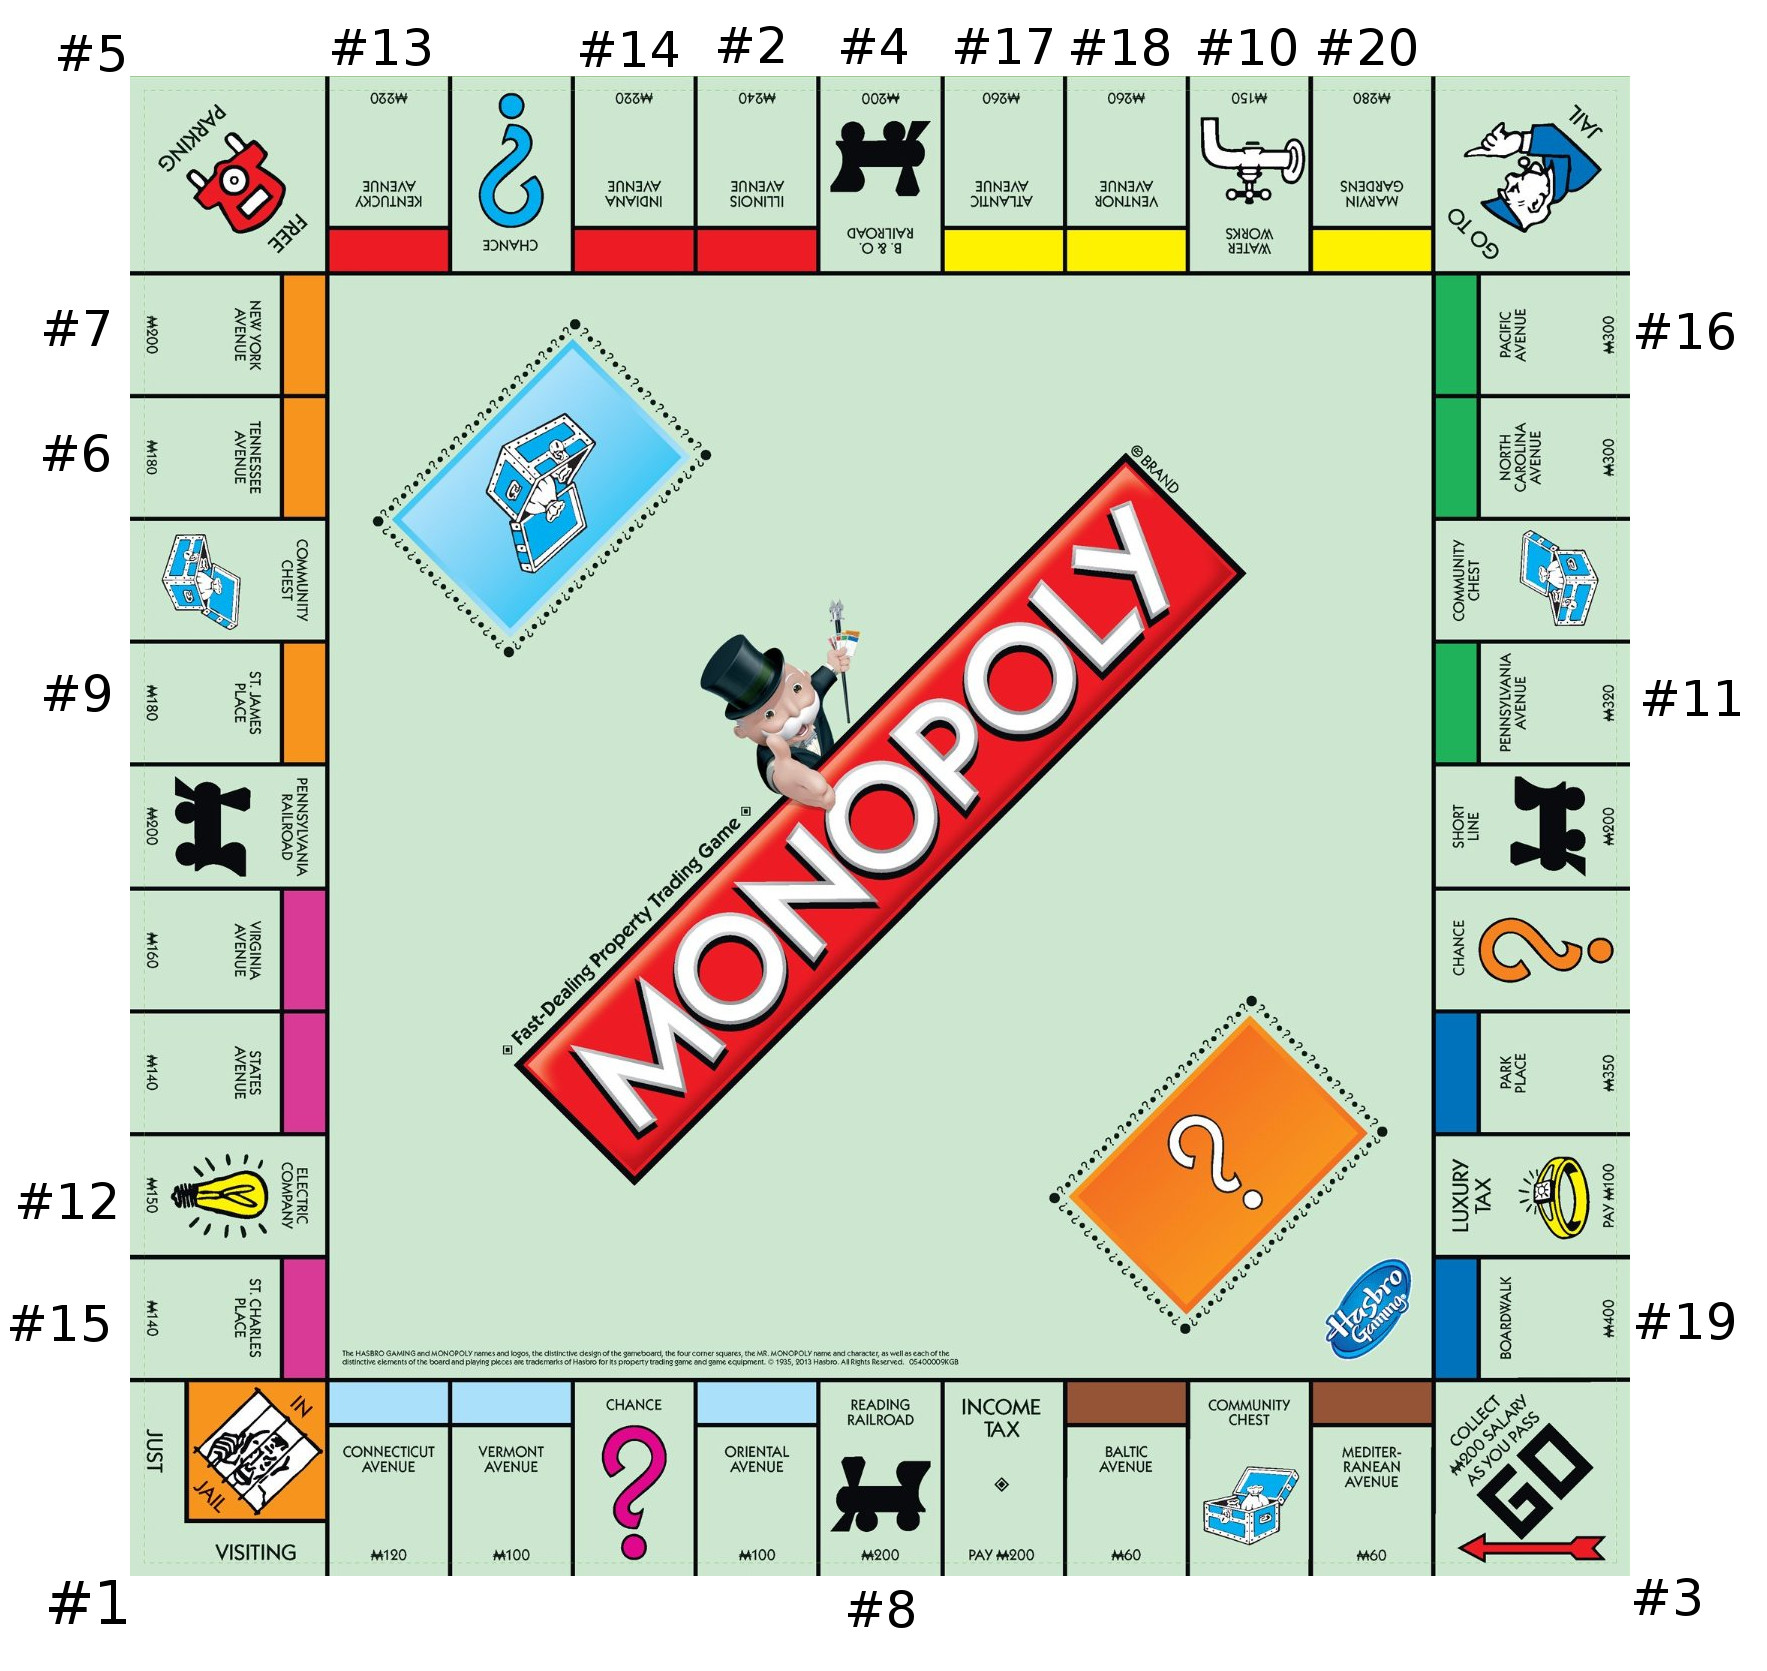
\includegraphics[width=0.75\textwidth]{tile_outcome.jpg}
\end{align*}

\subsubsection{Probabilistic Outcome}
Given that the expected value of two dice is 7, it is optimal to purchase as per a threshold of +7 tiles with respect to turn from the jail tile in order to gain the maximum probability of other players landing on it. By maximising the probability of other players landing on tiles owned by the player himself, there is a higher cumulative frequency for receiving rent and the chance of inflicting bankruptcy on others. Note that the second most probabilistic tile is a total of 14 tiles away from jail, which over two rolls corresponds to $4 \cdot E[X]$, or $4\cdot 3.5$. What is interesting to note is the fact that the lowest probability on the map is also an expected value of the initial dice rolls from \emph{Go}.
%expand on this?

\subsection{Further Expansion}
Given the probabilistic outcome strategy for individual tiles through Markovian logic, it is possible to extend this theory to developing property within the game. Given a probability of landing on a certain tile within a turn as the outcome of two dice, the following inequality must be satisfied in order to ensure a steady income and a lack of bankruptcy:
$$Income \geq Cost$$
This begets an expansion of what revenue really pertains to:
$$p(n)\cdot Rent\cdot E[X] \cdot n \geq Cost$$
Whereby on reordering becomes:
$$n = \left(\frac{Cost}{p(n)\cdot Rent\cdot E[X]}\right)$$
Where $n$ is the current turn of play. Given that properties have the potential to be developed when all three tiles within the colour group are owned, this causes the potential for bankruptcy to increase on landing on a developed tile as rent now increases proportionally with respect to the tile's state of development.
\section{Conclusion}
Overall a traditional game of Monopoly pertains to probabilistic rules governed by Markovian processes and dice theory. Through simulation and comparison with theory, features that were predicted to occur, were seen through Markov Chain probability matrices. Simulations and theory taken from studies on Monopoly games will differ slightly in comparison to this study, as dice may contain bias by having defects, as well as the addition of money and other players to play against. Simulations for determining the probability of landing on squares were on a single player, infinite rolls basis which is not true to actual gameplay; but nonetheless, provides a good basis for theory on understanding the influence of factors within a game, as well as that of seeing how each tile is not equal, and therefore choices of property determined by Markovian processes can be interpolated to improve chances of winning.
\section{Source Code}

\section{Bibliography}
\begin{thebibliography}{9}

\bibitem{bewersdorffj}
  Jorg Bewersdorff,
  \emph{Luck, Logic, and White Lies: The Mathematics of Game},
  A K Peters (2005),
  106-120.
\bibitem{snellj}
  J. Laurie Snell,
  \emph{Finite Markov Chains and their Applications},
  The American Mathematical Monthly (1959),
  66 (2),
  99-104.
\bibitem{ashr}
  R. B. Ash,
  \emph{Basic Probability Theory},
  (1970),
  Chapter 7.
\bibitem{bradym}
  Maxine Brady,
  \emph{The Monopoly Book},
  D. McKay, 
  (1974).
\bibitem{fellerw}
  W Feller,
  \emph{An Introduction to Probability Theory and Its Applications, Vol. 1},
  Wiley (1950).
\bibitem{hentzeli}
  Irving R. Hentzel,
  \emph{How to Win at Monopoly},
  Saturday Review of the Sciences,
  (April 1973),
  44-48.
\end{thebibliography}
\end{document}
